
% This thesis template is based on the report class of
% latex. Yout do not need to change this.
\documentclass[12pt, a4paper]{report}

% This includes all variables that are used in this work
% Use this document to specify your name, your reviewers
% and other values that you would like to maintain
% in one place.
\newcommand\myname{Adam Liscak}
\newcommand\mypkz{1810653053}

\newcommand\myfirstreviewer{Prof. (FH) Dr. Mario Döller}
% Leave second review empty for bachelor's thesis
%\newcommand\mysecondreviewer{Lukas Demetz, PhD}

\newcommand\mytitle{ Applying Real-Time Image Recognition Within Embedded Devices via Tensorflow and Keras Libraries }

% The value below is the date that you finished your work. This
% date appears on you work's cover page and in the "Eidesstattliche
% Erklärung".
\newcommand\mydate{06. July 2020}

% For a master's thesis use MA as type, BA for a bachelor's thesis
\newcommand\type{BA}

% Set the name of your study program. 
% DSIA for Data Science & Intelligent Analytics
% WEB for Web Business & Technology
% WCIS for Web Communications and Information Systems
\newcommand\program{WEB}

% Define the language in which you write this thesis
% Use DE for German, EN for English
\newcommand\lang{EN}


% This includes all packages and presets. You do not need
% to change this file unless you want to add new packages
% or change the presets of one of the used packages.
\usepackage{pxfonts}
\usepackage[T1]{fontenc}
\usepackage{graphicx}
\usepackage[utf8]{inputenc}
\usepackage{blindtext}  % Used for dummy text segments
\usepackage{natbib}
\usepackage{hyperref}
\usepackage{booktabs}
\usepackage{xcolor}
\usepackage{ifthen}
\usepackage{xspace}

\ifthenelse{\equal{\lang}{DE}}{
    \usepackage[ngerman]{babel} 
}{
    \usepackage[english]{babel} 
}

\usepackage{listings}
\lstset{numberbychapter=false}
\iflanguage{english}{\renewcommand{\lstlistlistingname}{List of Listings}}{\renewcommand{\lstlistlistingname}{Listingsverzeichnis}}

\usepackage{fancyhdr}  % Head and footer styling
\fancyhead[RO]{\thepage}
\fancyhead[LO]{\nouppercase\leftmark}
\renewcommand\headrulewidth{0.5pt}
\renewcommand\footrulewidth{0pt}

\usepackage[a4paper, left=3.5cm, right=3cm, top=3.5cm, bottom=3cm]{geometry}
\setlength{\headheight}{15pt}

\usepackage[title, titletoc, header]{appendix}
\renewcommand{\appendixname}{Appendix}

\usepackage{titlesec}
\titleformat{\chapter}{\bf \LARGE}{\thechapter.}{16pt}{\LARGE}

\usepackage{chngcntr}
\counterwithout{figure}{chapter}
\counterwithout{table}{chapter}

% Check for work type
\ifthenelse{\equal{\type}{MA}}{
    \newcommand\academictitle{Master of Science in Engineering (M.Sc.)}
    \newcommand\worktype{Masterarbeit\xspace}
}{
    \newcommand\academictitle{Bachelor of Science in Engineering (B.Sc.)}
    \newcommand\worktype{Bachelorarbeit\xspace}
}

% Check for study program

\ifthenelse{\equal{\program}{DSIA}}{
    \newcommand\studyprogram{Data Science \& Intelligent Analytics}
}{
    \ifthenelse{\equal{\program}{WEB}}{
        \newcommand\studyprogram{Web Business \& Technology}
    }{
        \newcommand\studyprogram{Web Communications \& Information Systems}
    }
}

\pagestyle{headings}
\setlength{\parindent}{0em}
\setlength{\parskip}{1.5em}
\renewcommand{\baselinestretch}{1.13}

\newcommand\frontmatter{
    \pagestyle{fancy}
    \fancyfoot{}
    \pagenumbering{Roman}
}

\newcommand\mainmatter{
    \pagenumbering{arabic}
}

\newcommand\backmatter{
    \pagenumbering{arabic}
    \renewcommand{\thepage}{A\arabic{page}}
}        

\lstset{
    numberstyle=\tiny,
    numbers=left,
    showstringspaces=false,
    breaklines=true,
    commentstyle=\itshape\color{darkgray},
    basicstyle=\ttfamily,
    stringstyle=\color{orange},
    keywordstyle=\bf\color{green!40!black},
    identifierstyle=\color{blue}
}

\hypersetup{
  pdftitle    = \mytitle,
  pdfsubject  = \worktype,
  pdfauthor   = \myname,
  pdfcreator  = {pdflatex using template provided by University of Applied Sciences FH Kufstein Tirol},
  bookmarksnumbered = true,
  colorlinks = true,
  linkcolor = blue,
  citecolor = green,
  urlcolor = orange
}


% This includes custom latex commands. You can use this
% file to create your own command sequences.
\newcommand{\fh}{\textsc{FH Kufstein Tirol}}

\newcommand{\fig}[4]{
    \begin{figure}[ht]
        \centering
        \includegraphics[width=#4\textwidth]{#1}
        \caption{#2}
        \label{#3}
    \end{figure}
}


% If you want to print your thesis in black and white
% uncomment the following section

% \hypersetup{
%     colorlinks=false,
%     pdfborder = 0 0 0
% }
% \lstset{
%     commentstyle=\itshape,
%     basicstyle=\ttfamily,
%     stringstyle=\color{black},
%     keywordstyle=\bf,
%     identifierstyle=\color{black}
% }

\begin{document}

    \frontmatter

    % This places the front matter. You do not need to 
    % change this file. All thesis-specific values are 
    % imported from "variables.tex".
    \begin{titlepage}
 
    \vfill
    \begin{center}
      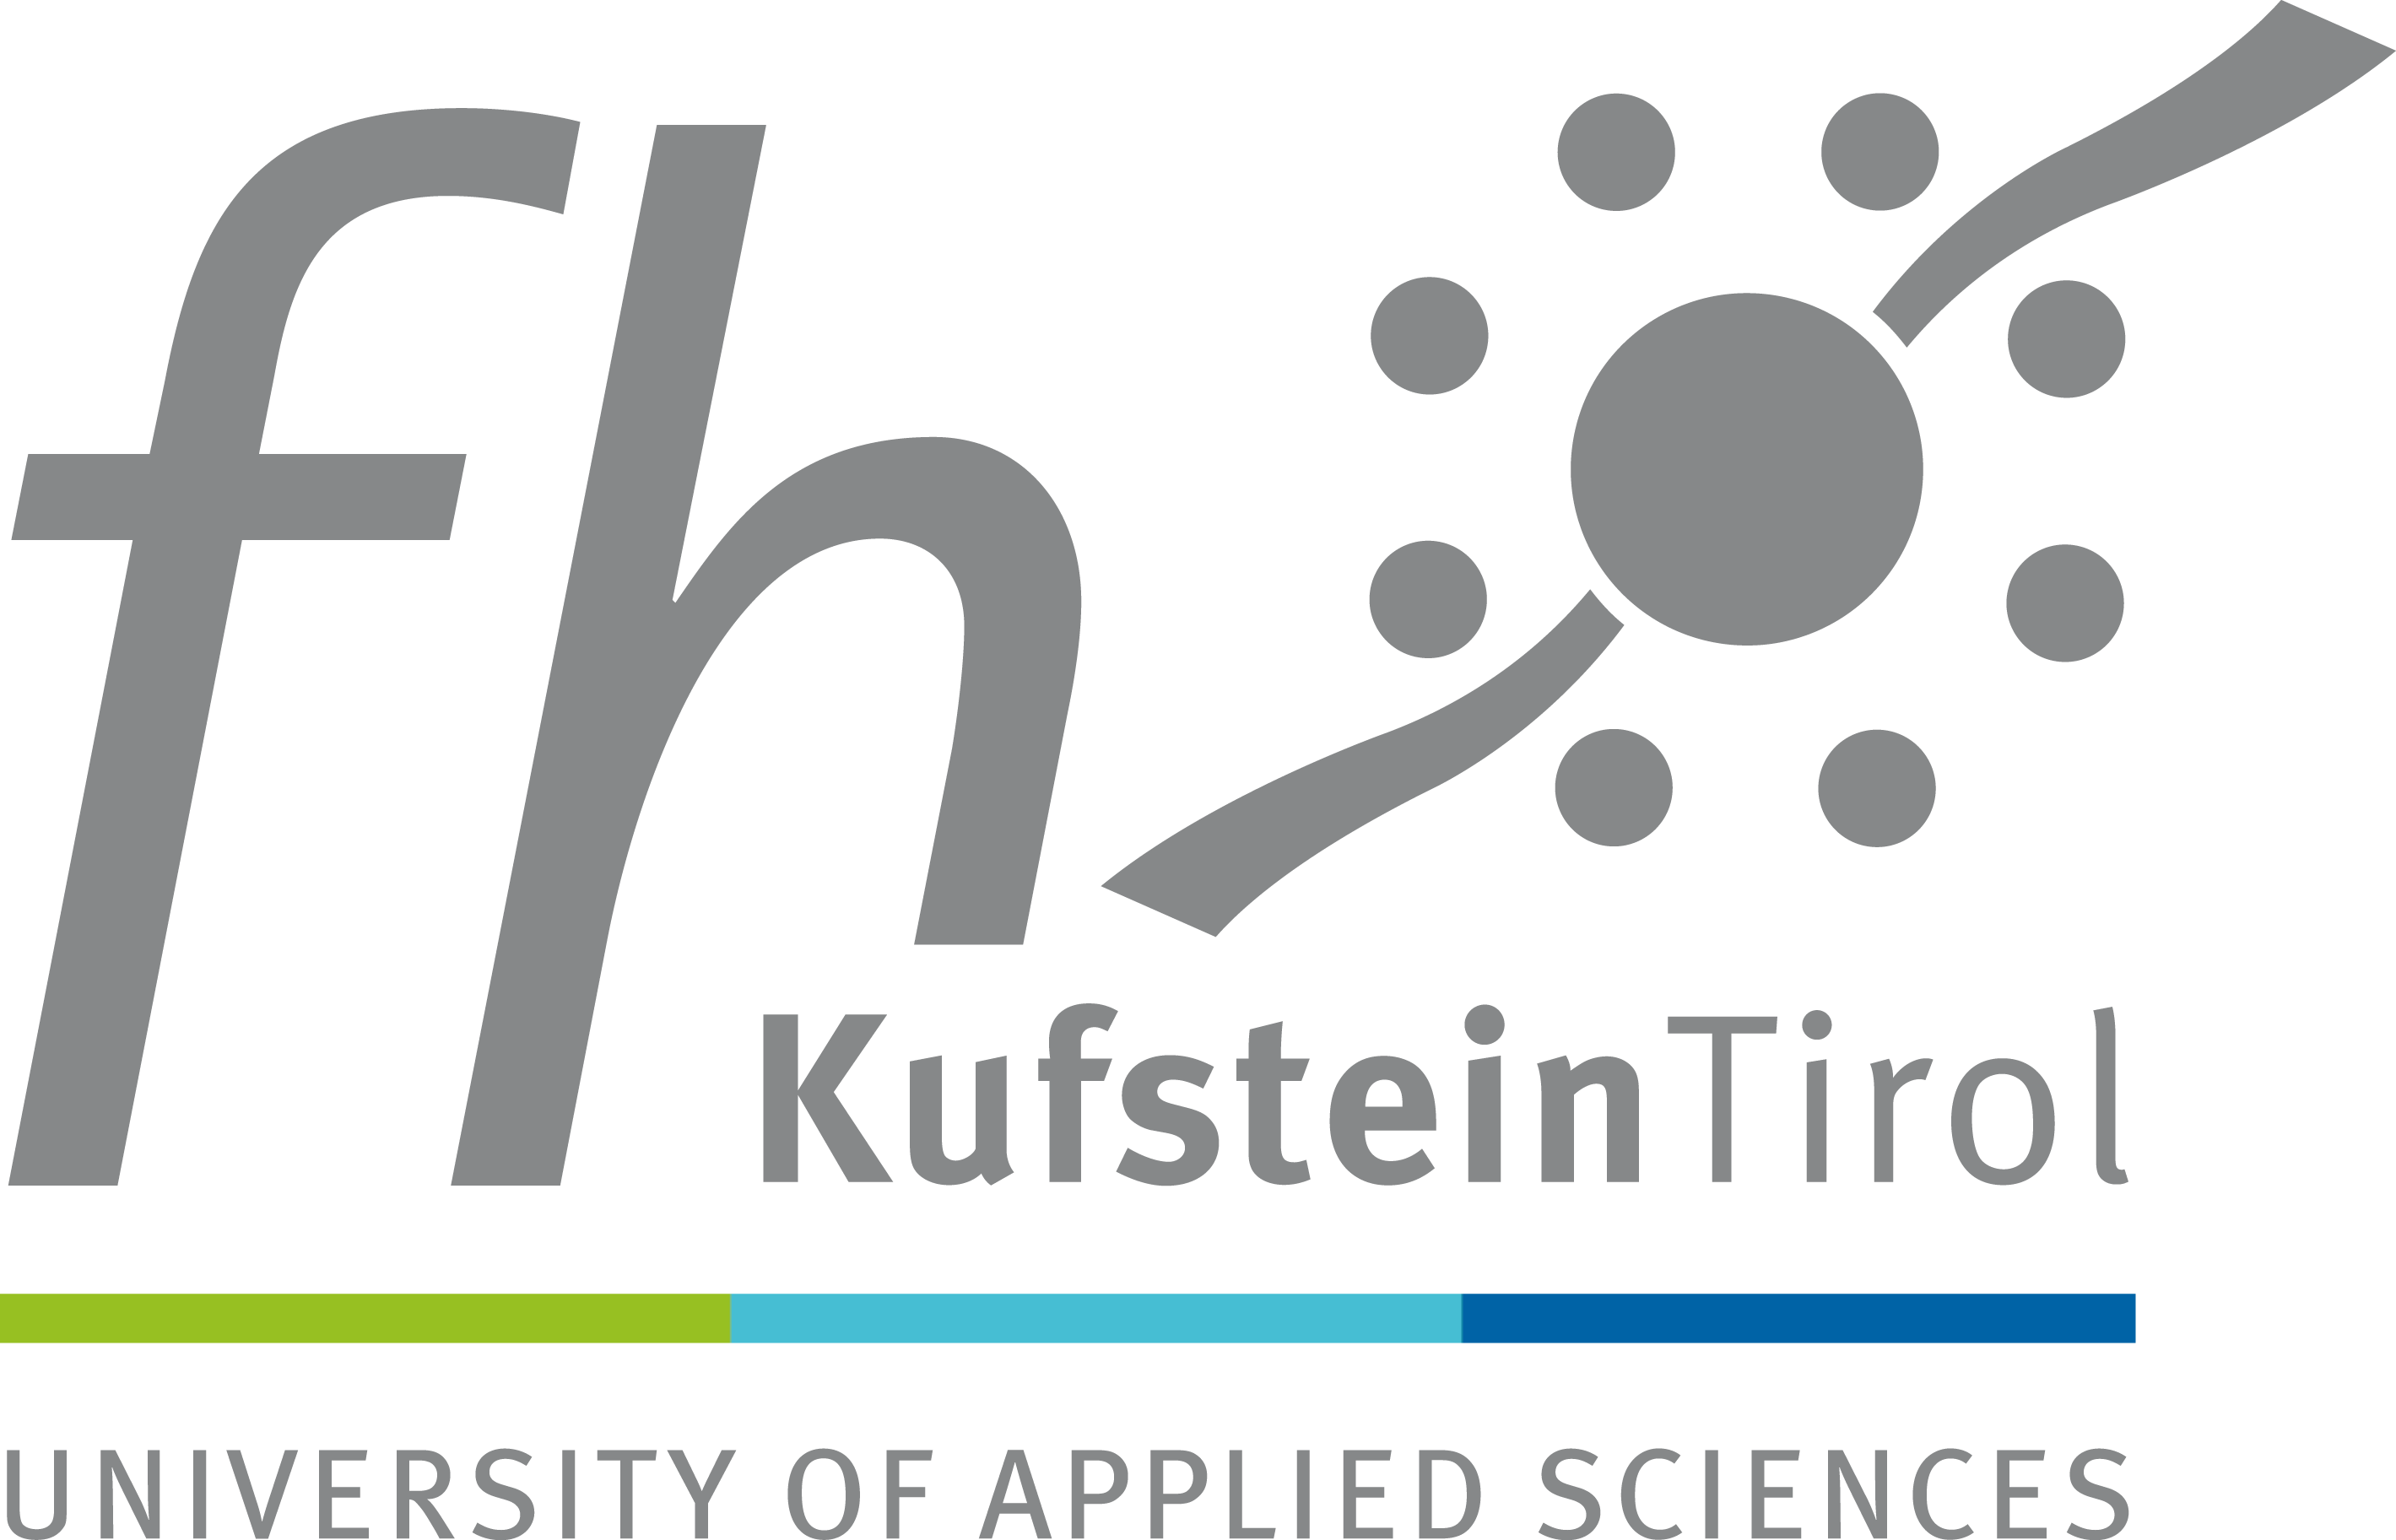
\includegraphics[width=4.5cm]{img/kufstein_logo.png} \\ 
    \end{center}
    \vfill
  
    \begin{center}
      \Large \textbf{\mytitle}
    \end{center} 
    \vfill
  
    \begin{center}
      %\condMASTER{\Large Masterarbeit}{\Large Bachelorarbeit}
      \worktype
    \end{center}
    \vfill
  
    \begin{center}
      zur Erlangung des akademischen Grades\\
      \large \textbf{\academictitle}
    \end{center}
    \vfill
  
    \begin{center}
      Eingereicht bei:\\ 
      \vspace{0.1cm}
      \large \textbf{Fachhochschule Kufstein Tirol Bildungs GmbH}\\
      \vspace{0.1cm}
      \large \textbf{\studyprogram}
    \end{center}
    \vfill
  
    \begin{center}
      Verfasser/in:\\
      \vspace{0.1cm}
      \large \textbf{\myname}\\
      \vspace{0.1cm}
      \large \textbf{\mypkz}\\
    \end{center}
    \vfill
  
    \begin{center}
      \begin{tabular}{lll}
        \ifthenelse{\equal{\type}{MA}}{
          Erstgutachter  & : & \myfirstreviewer \\
          Zweitgutachter & : & \mysecondreviewer
        }{
          Gutachter  & : & \myfirstreviewer \\
        }
      \end{tabular}
    \end{center} 
    \vfill
  
    \begin{center}
      Abgabedatum: \\
      \vspace{0.1cm}
      \large \textbf{\mydate}
    \end{center} 
    \vfill  
  \end{titlepage}


    % This places the "Eidesstattliche Erklärung". This 
    % Document is always in German, even if your work is
    % written in English.
    \chapter*{Eidesstattliche Erklärung}
\thispagestyle{empty}

Ich erkläre hiermit, dass ich die vorliegende \worktype selbständig und ohne fremde Hilfsmittel verfasst und in der Bearbeitung und Abfassung keine anderen als die angegebenen Quellen oder Hilfsmittel benutzt sowie wörtliche und sinngemäße Zitate als solche gekennzeichnet habe. Die vorliegende \worktype wurde nicht anderweitig für Prüfungszwecke vorgelegt.

\vspace{2cm}
Kufstein, \mydate

\vspace{2cm}
\rule{10cm}{1pt}\\
\myname{}



    % This will include a "Sperrvermerk". This document
    % is always in German, even if your work is written
    % in English. Please remove this line, if necessary.
    \chapter*{Sperrvermerk}
\thispagestyle{empty}

Ich habe die Sperrung meiner \worktype beantragt, welche von der Studiengangsleitung genehmigt wurde.

\vspace{2cm}
Kufstein, \mydate

\vspace{2cm}
\rule{10cm}{1pt}\\
\myname{}


    % This inserts all necessary tables into your work.
    \tableofcontents
    \listoffigures
    \listoftables

    % Use this if you have any code listings
    \lstlistoflistings

    % This adds a german and an english summary to your work.
    % You always have to add both, independent of whether your
    % work is done in german or english
    \thispagestyle{empty}

\textbf{FH Kufstein Tirol\\\studyprogram}

Abstract of the thesis: \textbf{\mytitle}

\textbf{Author:} \myname\\
\ifthenelse{\equal{\type}{MA}}{
    \textbf{First reviewer:} \myfirstreviewer\\
    \textbf{Second reviewer:} \mysecondreviewer\\
}{
    \textbf{First reviewer:} \myfirstreviewer\\
}

\thispagestyle{empty}

\textbf{FH Kufstein Tirol\\\studyprogram}

Abstract of the thesis: \textbf{\mytitle}

\textbf{Author:} \myname\\
\ifthenelse{\equal{\type}{MA}}{
    \textbf{First reviewer:} \myfirstreviewer\\
    \textbf{Second reviewer:} \mysecondreviewer\\
}{
    \textbf{First reviewer:} \myfirstreviewer\\
}

\thispagestyle{empty}

\textbf{FH Kufstein Tirol\\\studyprogram}

Abstract of the thesis: \textbf{\mytitle}

\textbf{Author:} \myname\\
\ifthenelse{\equal{\type}{MA}}{
    \textbf{First reviewer:} \myfirstreviewer\\
    \textbf{Second reviewer:} \mysecondreviewer\\
}{
    \textbf{First reviewer:} \myfirstreviewer\\
}

\input{chapters/summary_en}

% End with date
\mydate{}


% End with date
\mydate{}


% End with date
\mydate{}

    % !TEX root =../document.tex
% Your text goes here (aprox. 350 words)
\Blindtext[2][1]


    \mainmatter

    % This places the actual chapters. The files referenced here
    % are just an example. You can add additional chapters if 
    % necessary
    % !TEX root =../document.tex
\chapter{Introduction}

\blindtext \citet{Shearer2000}

\section{Problem Situation}

\blindtext

\fig{img/sax_approximated_series}{Sax approximation of a time series}{fig:sax}{0.5}

As can be seen in Figure~\ref{fig:sax} \ldots

\section{Objectives}

\blindtext

\section{Methods}

\blindtext

\section{Structure}

\blindtext

\section{Tables}

Table~\ref{tab:table-one} shows an example table.

\begin{table}[htbp]
    \centering
    \caption{This is a table}
    \label{tab:table-one}
    \begin{tabular}{lll}
        \addlinespace
        \toprule
        Column 1 & Column 2 & Column 3 \\
        \midrule
        A     & B     & C \\
        D     & E     & F \\
        G     & H     & I \\
        \bottomrule
    \end{tabular}
\end{table}

\section{Source Code}

\begin{lstlisting}[language=Java, caption=Hello World in Java, label=lst:hello-world-java]
public class Hello {
    public static void main(String[] args) {
        System.out.println("Hello World");
    }
}
\end{lstlisting}

Listing~\ref{lst:hello-world-java} shows the classic Hello World in Java.

\lstinputlisting[language=Python, caption=Hello World in JavaScript, label=lst:hello-world-py]{./lst/hello.py}

Listing~\ref{lst:hello-world-py} shows the classic Hello World in Python.

    \chapter{Foundations}

\blindtext[1]

\section{Machine Learning}

\Blindtext[4][1]

\section{Deep Learning}

\Blindtext[4][1]

    % !TEX root =../document.tex
\chapter{Pattern Recognition with Deep Neural Networks}
Hello world

\Blindtext[4][1]

    \chapter{Neural Networks on Embedded Devices}

\Blindtext[4][1]

    % !TEX root =../document.tex
\chapter{Discussion}

\Blindtext[4][1]


    \bibliographystyle{apalike}

    % This places the bibliography. You can add more
    % bibliographic items it the bibliography.bib file. 
    % We suggest using a reference manager (e.g., Jabref)
    % to maintain this file
    \bibliography{bibliography}

    \newpage
    
    \backmatter

    \begin{appendices}

        % This is the actual appendix. The files referenced here
        % are just examples. You can add additional appendices
        % if necessary
        \chapter{List of Interview Partners}

\Blindtext[2][6]

        \chapter{Code Table}

\blindtext


    \end{appendices}

\end{document}
